\chapter{User Studies}

\section{User Test at the Digital Arts
Exhibition}\label{user-test-at-the-digital-arts-exhibition}

\begin{figure}[htbp]
\centering
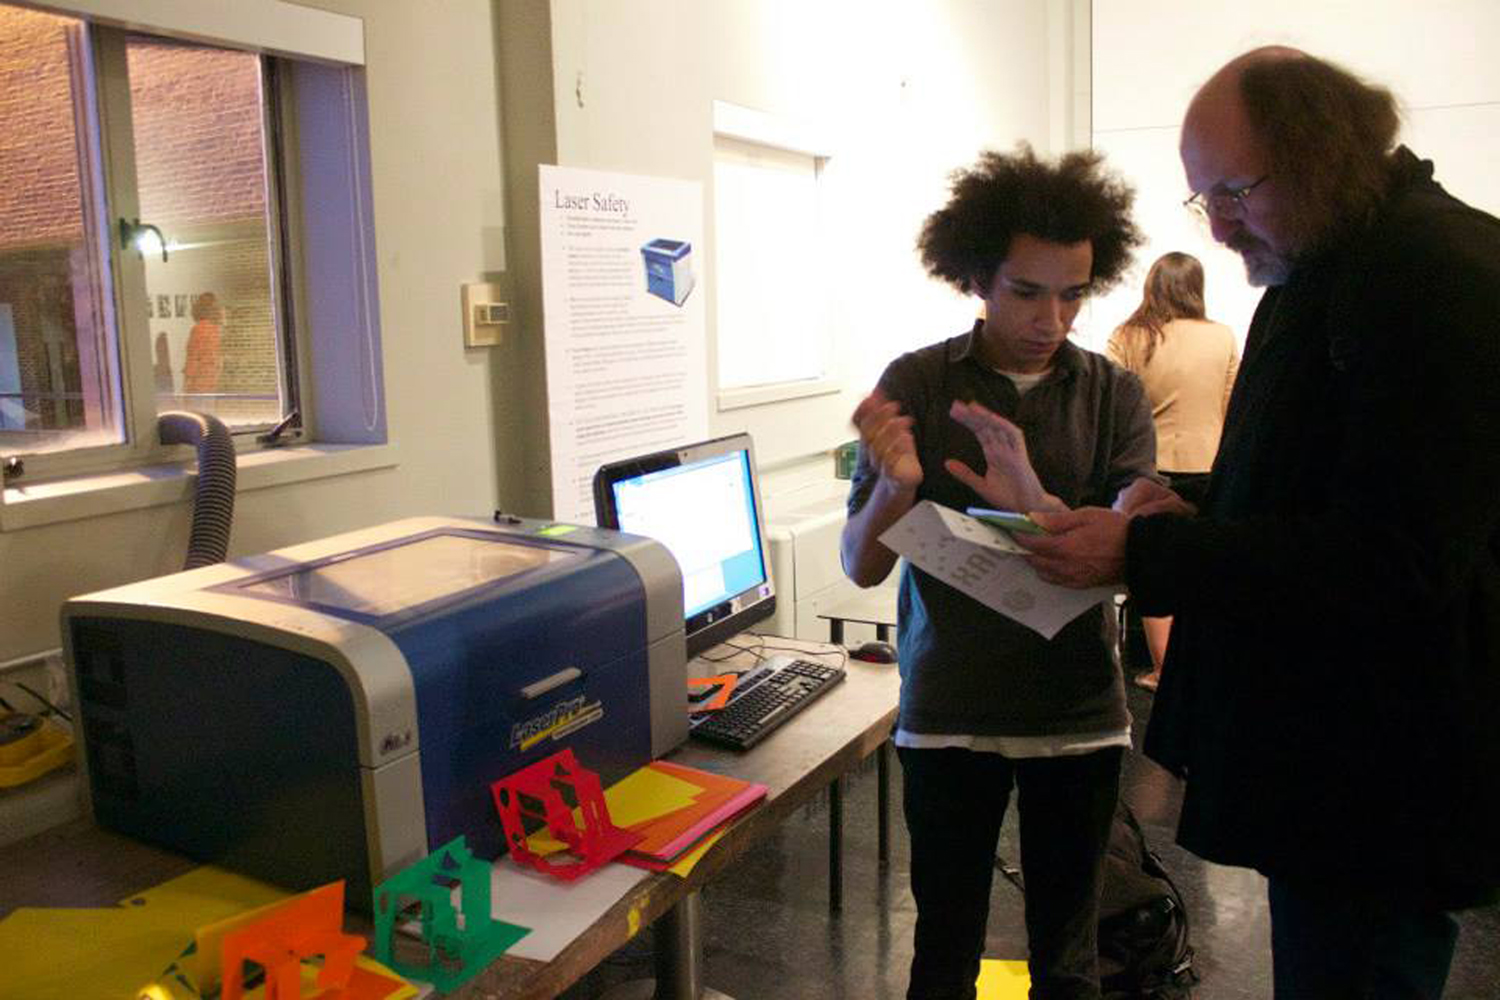
\includegraphics{figures/50_User_Study_Dax/dax_facebook_credit_Julietta_Gervase}
\caption{Foldlings at the Digital Arts Exhibition.
\textbf{\textgreater{}\textgreater{}TODO: photo credit Julietta
Gervase}}
\end{figure}

On April 28, 2015, we tested our system with attendees of the Digital
Arts Exhibition at Dartmouth. After a brief demonstration of how to
create folds and preview their design, users designed cards using
Foldlings. Users drew sketches and then sent an email containing an SVG
file to the computer connected to the laser cutter. Finally, they placed
a piece of paper in the laser cutter, and watched as the laser beam cut
out their design. Over the course of two hours, users cut and folded 31
popup cards. \textbf{\textless{}\textless{}TOOO: CITE DAX
\textless{}\textless{}TODO:}

The system we demonstrated at the exhibition was incomplete --- it
contained the basic box fold and freeform shape tools, but did not
include some advanced features of the final software, such as dragging
folds or shading based on plane orientation. The alpha software also
contained several bugs that disrupted the experience. However, the
system was usable enough for people to create cards, and observing user
behavior was invaluable in designing our final product.

Because users were new to our system --- and constrained by the pressure
of other users waiting to design cards --- designs were relatively
simple. Sketches generally contained between 2 and 5 fold features in
addition to the base card --- the most complex design contained 10 fold
features. Despite their simplicity, sketches showed a wide range of
designs, ranging from abstract shapes to representational scenes ---
users sketched symbols, Chinese characters, and geometric forms. Most of
the sketches utilized both freeform and box fold features, mixing the
two element types to create a composition. One of the most popular
design elements was the user's name: 5 of the cards contained names or
initials. Roughly a third of the designs took advantage of nesting ---
constructing fold features inside each other.

Because users were able to quickly design and fabricate their design,
people generally left satisfied. People typically spent around 20
minutes at our booth, leaving with a popup card they had created.
However, the experience was not frictionless. Users were frustrated by
crashes: touching the screen with more than one finger or drawing while
calculating planes were the most common reasons for failure. Other
common complaints were the lack of a delete/undo button and that the UI
did not show which tool was currently selected.

Folding the fabricated design also presented difficulties. Although they
were able to see a 3d preview of their design while creating it, users
had often relinquished the iPad by the time they folded their design.
They were often unsure how to fold their card, and struggled to discover
the correct fold orientations. In some cases, it took longer for users
to fold their creation than to design it.

We observed several unexpected behaviors. A few users rotated the screen
to design a card in a landscape view, rather than the portrait
orientation implied by the orientation of the buttons and 3d preview.
They used this orientation to design cards that folded medially rather
than laterally. Several users also constructed overlapping features by
drawing on top of existing features. These features did not simulate
correctly, as they intersected with existing edges. However, this
behavior demonstrated a desire to construct more complex geometry. In
the final software we implement unions for fold features --- the most
recently-drawn feature occludes features underneath it, modifying their
edges.

Users also relied on the 3d preview to differing degrees. Some users
viewed the preview after every operation, while others only switched to
the preview occasionally. Many users relied on the 3d preview as a
reference to how to fold their popup card. We were surprised by this,
and conducted further user studies to determine the effectiveness of
methods of displaying 3d information.
